\chapter*{Pause Synthèse : Dérivées et Primitives}
\addcontentsline{toc}{chapter}{Pause Synthèse : Dérivées et Primitives}

Cette pause a pour but de clarifier le lien fondamental entre le calcul différentiel (dérivées) et le calcul intégral (primitives), deux piliers de l'analyse.

\section*{1. Le Lien Fondamental}

La dérivation et l'intégration sont deux opérations \textbf{inverses} l'une de l'autre (à une constante près).

\begin{center}
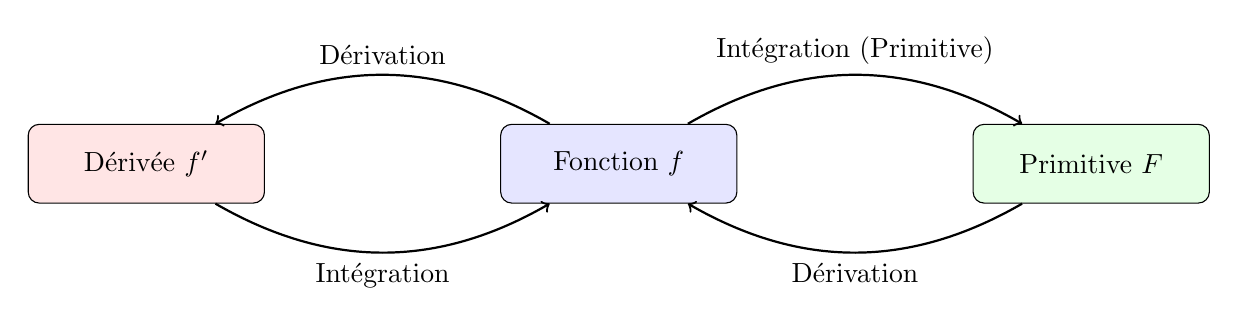
\begin{tikzpicture}
    \node[draw, rectangle, rounded corners, fill=blue!10, minimum width=3cm, minimum height=1cm] (f) at (0,0) {Fonction $f$};
    \node[draw, rectangle, rounded corners, fill=green!10, minimum width=3cm, minimum height=1cm] (F) at (6,0) {Primitive $F$};
    \node[draw, rectangle, rounded corners, fill=red!10, minimum width=3cm, minimum height=1cm] (df) at (-6,0) {Dérivée $f'$};

    \draw[->, thick, bend left] (f) to node[above] {Intégration (Primitive)} (F);
    \draw[->, thick, bend left] (F) to node[below] {Dérivation} (f);
    
    \draw[->, thick, bend right] (f) to node[above] {Dérivation} (df);
    \draw[->, thick, bend right] (df) to node[below] {Intégration} (f);
\end{tikzpicture}
\end{center}

\section*{2. Tableau Comparatif}

\begin{center}
\begin{tabular}{|c|c|c|}
\hline
\textbf{Opération} & \textbf{Dérivation} & \textbf{Intégration (Primitive)} \\
\hline
\textbf{Notation} & $f'(x)$ & $F(x) = \int f(x) dx$ \\
\hline
\textbf{Sens Physique} & Vitesse instantanée & Distance parcourue (cumul) \\
\hline
\textbf{Sens Géométrique} & Pente de la tangente & Aire sous la courbe \\
\hline
\textbf{Unicité} & Unique & Une infinité (à une constante $k$ près) \\
\hline
\textbf{Calcul} & Règles mécaniques ($uv, u/v...$) & Nécessite astuce ou reconnaissance de forme \\
\hline
\end{tabular}
\end{center}

\section*{3. Lecture du Tableau des Usuelles}

Le tableau des primitives n'est rien d'autre que le tableau des dérivées lu \textbf{à l'envers}.

\begin{itemize}
    \item \textbf{Dérivée :} On part de $f$ pour trouver $f'$.
    \item \textbf{Primitive :} On a $u'$ et on cherche $u$. C'est pourquoi il est crucial de reconnaître la forme $u' \times (\dots)$.
\end{itemize}

\begin{regleredaction}
Pour calculer une intégrale ou trouver une primitive, posez-vous toujours la question : 
\textbf{"De qui cette fonction est-elle la dérivée ?"}
Si la réponse n'est pas évidente, cherchez à faire apparaître une forme connue du tableau ($u'u^n, u'/u, u'e^u \dots$).
\end{regleredaction}
